%%%%%%%%%%%%%%%%%%%%%%%%%%%%%%%%%%%%%%%%%%%%%%%%%%%%%%%%%%%%%%%%%
\chapter{BULGULAR}\label{CH4}
%%%%%%%%%%%%%%%%%%%%%%%%%%%%%%%%%%%%%%%%%%%%%%%%%%%%%%%%%%%%%%%%%

Bu bölümde Bölüm \ref{CH3}'te açıklanan deneylerin sonuçları, araştırma sorularının sırasıyla sunulmaktadır. Bölüm \ref{sec:res:piroi}--\ref{sec:res:defense} saldırı ve savunma deneylerini, Bölüm \ref{sec:res:fovinfo}--\ref{sec:res:generalization} önerilen FoveaHE yönteminin deneylerini kapsar. Meta veri saldırısında AUC değerleri 5 tohumun ortalamasıdır. Bağlam saldırısının ana görüşlerinde ve çözüm deneylerinin ana yapılandırmalarında 5 tohumun ortalaması ve standart sapması, diğer CNN tabanlı deneylerde tek tohum değerleri verilmiştir.

\section{$\Pi_{\mathrm{ROI}}$ Yeniden Üretiminin Doğruluğu ve Maliyeti}\label{sec:res:piroi}

\textbf{Doğruluk.} Seçici şifreli hesaplama, gerçek görüntü ve gerçek ROI maskeleriyle şifresiz hesaplamayla aynı sonucu vermiştir. Beyin MR örnek görüntüsünde tümör maskesiyle ($\rho = 0.018$) en büyük mutlak hata $64 \times 64$ çözünürlükte $4.7 \times 10^{-6}$, $128 \times 128$ çözünürlükte $9.2 \times 10^{-6}$ olmuştur. Göğüs röntgeni örnek görüntüsünde akciğer maskesiyle ($\rho = 0.20$) bu değerler sırasıyla $6.7 \times 10^{-6}$ ve $1.7 \times 10^{-5}$'tir. Bu hatalar CKKS'in yaklaşık aritmetiğinin doğal düzeyindedir. Buradaki $\rho$ değerleri tek bir örnek görüntüye aittir; Çizelge \ref{tbl:saldiriB}'teki gizli alan oranları tüm görüntülerin, Çizelge \ref{tbl:savunma}'daki oranlar ise savunma deneyinin test görüntülerinin ortalamasıdır ($224 \times 224$ çözünürlükte).

\textbf{Maliyet.} Çizelge \ref{tbl:maliyet} ve Şekil \ref{fig:piroi}, şifreli alan oranına göre maliyeti göstermektedir. Hız kazancını belirleyen temel etken şifreli metin sayısıdır. $64 \times 64$ görüntünün tamamı tek bir şifreli metne sığdığı için bu çözünürlükte seçici şifreleme anlamlı bir hızlanma sağlamamıştır; ölçülen oranlar $0.71$ ile $1.35$ kat arasında ve ölçüm gürültüsü düzeyindedir. $512 \times 512$ görüntülerde hız kazancı \%1 ROI'de 27.4 kata ulaşmış, \%25 ROI'de 3.88 kata inmiştir. Bu ikinci değer, $\Pi_{\mathrm{ROI}}$ makalesinde aynı oran için bildirilen 4.07 katlık kazançla uyumludur \cite{bakas2026roi}. Makalede \%1 ROI için bildirilen 84 katlık kazanç ise bizim ölçümümüzden yüksektir. Farkın büyük kısmı tam şifreli hesaplamadan gelmektedir: makale $512 \times 512$ görüntü için tam şifreli sunucu hesaplamasına 1048 saniye bildirirken bizim ölçümümüzde bu süre 41.2 saniyedir (yaklaşık 25 kat); \%1 ROI'de ise süreler 12.4 ve 1.49 saniyedir (yaklaşık 8 kat). Makalenin kodu yayımlanmadığı için bu farkın kaynağı kesin olarak bilinmemektedir. Muhtemel nedenler, bizim uygulamamızda tam şifreli hesaplamanın yoğun paketleme ve 2'nin kuvvetine tamamlama ile daha verimli yapılması, modül zincirinin bir seviye kısa olması (Bölüm \ref{sec:ckks}) ve donanım farkıdır. Şifreli alan büyüdükçe kazanç hızla erimektedir: \%75 ROI'de 1.33, \%90 ROI'de 1.10 kat.

\begin{table*}[h!]
{\setlength{\tabcolsep}{4pt}
\caption{Şifreli alan oranına göre $\Pi_{\mathrm{ROI}}$ yeniden üretiminin maliyeti ($256 \times 256$ görüntüde 5, $512 \times 512$ görüntüde 3 tekrarın ortalaması; süre saniye, $\pm$ standart sapma).}
\begin{center}
\vspace{-6mm}
{\small
\begin{tabular}{cccccccc}
\hline\hline
& \multicolumn{3}{c}{$256 \times 256$} & \multicolumn{4}{c}{$512 \times 512$} \\
$\rho$ & Şifreli metin & Süre & Hız & Şifreli metin & Süre & Hız & Yükleme (MB) \\
\hline
0.01 & 1 & 1.33 & 8.01 & 1 & $1.52 \pm 0.00$ & 27.41 & 0.86 \\
0.05 & 1 & 1.51 & 7.03 & 2 & $2.89 \pm 0.01$ & 14.35 & 1.71 \\
0.10 & 1 & 1.61 & 6.61 & 4 & $5.30 \pm 0.00$ & 7.84 & 3.42 \\
0.25 & 2 & 2.89 & 3.67 & 8 & $10.70 \pm 0.13$ & 3.88 & 6.84 \\
0.50 & 4 & 5.47 & 1.94 & 16 & $20.95 \pm 0.13$ & 1.98 & 13.69 \\
0.75 & 7 & 8.83 & 1.20 & 24 & $31.29 \pm 0.15$ & 1.33 & 20.54 \\
0.90 & 8 & 10.61 & 1.00 & 29 & $37.63 \pm 0.03$ & 1.10 & 24.81 \\
1.00 & 8 & 10.62 & 1.00 & 32 & $41.54 \pm 0.10$ & 1.00 & 27.38 \\
\hline
\end{tabular}}
\vspace{-6mm}
\end{center}
\label{tbl:maliyet}}
\end{table*}

\begin{figure}[h!]
 \centering
 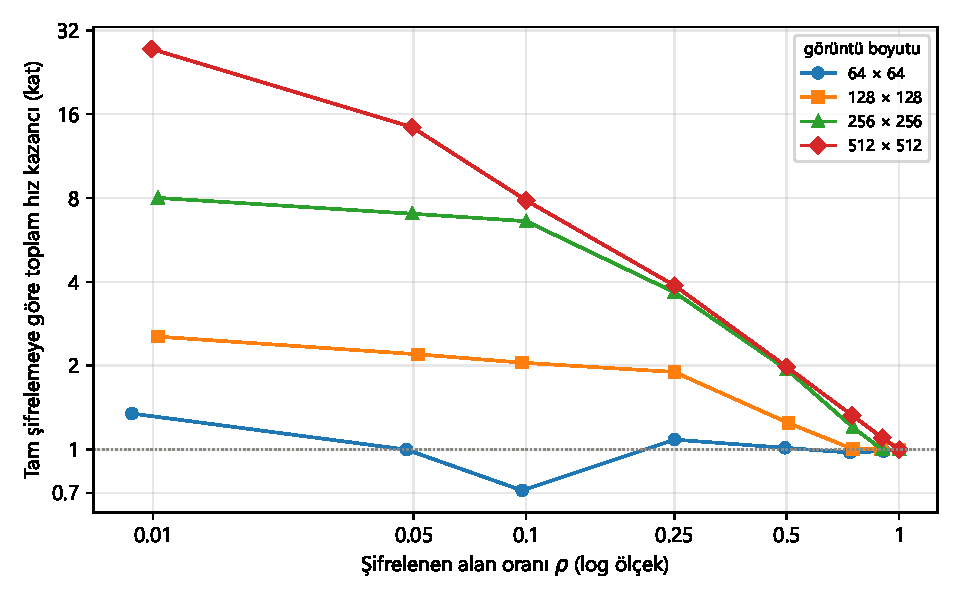
\includegraphics[width=12cm,keepaspectratio=true]{./fig/piroi_hiz_kazanci_tez.pdf}
 \caption{Tam homomorfik şifrelemeye göre toplam hız kazancının şifreli alan oranı ve görüntü boyutuyla değişimi (iki eksen de logaritmik ölçek; noktalı çizgi 1 kat).}
 \label{fig:piroi}
\end{figure}

\section{Saldırı A: ROI Meta Verisinin Sızıntısı}\label{sec:res:A}

Çizelge \ref{tbl:saldiriA}, yalnızca protokolün serbest bıraktığı meta veriyi kullanan saldırının sonuçlarını göstermektedir.

\begin{table*}[h!]
{\setlength{\tabcolsep}{4pt}
\caption{Yalnızca ROI meta verisi ve girdi boyutuyla teşhis tahmini (AUC).}
\begin{center}
\vspace{-6mm}
{\small
\begin{tabular}{lllccc}
\hline\hline
Veri & Hedef & ROI & Öznitelikler & AUC & \%95 GA \\
\hline
Beyin MR & Tümör tipi (3 sınıf) & Tümör & Girdi boyutu & 0.457 & 0.401--0.519 \\
 & & & Konum & 0.775 & 0.743--0.804 \\
 & & & Büyüklük & 0.708 & 0.674--0.736 \\
 & & & Şekil & 0.722 & 0.691--0.747 \\
 & & & Tümü & 0.830 & 0.801--0.855 \\
\hline
COVID-QU-Ex & Teşhis (3 sınıf) & Akciğer & Konum & 0.729 & 0.720--0.739 \\
 & & & Büyüklük & 0.765 & 0.757--0.775 \\
 & & & Şekil & 0.780 & 0.771--0.788 \\
 & & & Tümü & 0.834 & 0.827--0.841 \\
 & Normal / pnömoni & Akciğer & Tümü & 0.904 & 0.895--0.913 \\
 & Normal / COVID-19 & Akciğer & Tümü & 0.853 & 0.842--0.863 \\
 & Pnömoni / COVID-19 & Akciğer & Tümü & 0.832 & 0.820--0.842 \\
 & COVID-19 / diğer & Enfeksiyon & ROI alanı & 1.000 & -- \\
\hline
Kaggle & Normal / pnömoni & -- & Girdi boyutu & 0.934 & -- \\
 & Normal / COVID-19 & -- & Girdi boyutu & 0.920 & -- \\
\hline
\end{tabular}}
\vspace{-6mm}
\end{center}
\label{tbl:saldiriA}}
\end{table*}

Beyin MR verisinde tümörün konumu, büyüklüğü ve şekli birlikte tümör tipini makro AUC $0.830$ ile ele vermiştir. Sınıf bazında hipofiz tümörü AUC $0.949$, gliom $0.827$, meningiom $0.714$ ile ayırt edilmiştir. Permütasyon önemine göre en çok bilgi taşıyan öznitelik tümörün yatay ağırlık merkezidir (AUC düşüşü $0.102$). Bunu sınırlayıcı kutunun üst kenarı ($0.028$) ve kutu doluluğu ($0.023$) izlemiştir. Orta hatta yer alma, hipofiz tümörlerinin tipik konumuyla uyumludur. Bu veri kümesinde kesitlerin neredeyse tamamı aynı boyutta olduğundan girdi boyutu sızıntı yaratmamıştır (AUC $0.457$).

COVID-QU-Ex verisinde görüntülerin tamamı aynı çözünürlüğe getirildiği için yalnızca akciğer maskesinin geometrisi kullanılmıştır. Bu geometri teşhisi 3 sınıflı AUC $0.834$, normal ile pnömoni ayrımını AUC $0.904$ ile ele vermiştir. ROI'nin enfeksiyon maskesi olarak tanımlandığı uç durumda ROI alanı tek başına COVID-19 tanısını kusursuz biçimde ayırmıştır. Bu sonuç bir veri kümesi artefaktıdır: COVID-QU-Ex'in enfeksiyon alt kümesinde maskeler yalnızca COVID-19 görüntüleri için çizilmiş, COVID dışı pnömoni ve normal görüntülerin maskeleri boş bırakılmıştır (rastgele 150'şer örnekte COVID-19 maskelerinin tamamı dolu, diğerlerinin tamamı boştur). COVID dışı pnömonide de enfeksiyon bulunduğundan, klinik olarak eksiksiz etiketlenmiş bir kümede bu ayrımın bu kadar kolay olması beklenmez. Orijinal çözünürlüklerin korunduğu Kaggle kümesinde ise ROI geometrisine hiç bakmadan yalnızca görüntü boyutu normal ile pnömoniyi AUC $0.934$ ile ayırmıştır.

\textbf{Kesit yönü kontrolü.} Çizelge \ref{tbl:yon}, beyin MR verisinde konum sızıntısının kesit yönünden kaynaklanıp kaynaklanmadığını sınayan kontrolün sonuçlarını vermektedir. Yalnızca kesit yönü tümör tipini neredeyse hiç ele vermemiştir (AUC $0.540$). Buna karşın meta veri saldırısı her yönün kendi içinde de güçlü kalmıştır. Yön tahmininin görsel olarak en güvenilir olduğu sagital grupta AUC $0.891$'dir (Şekil \ref{fig:yon}). Dolayısıyla meta veri sızıntısı kesit yönünün bir yan etkisi değildir.

\begin{table*}[h!]
{\setlength{\tabcolsep}{12pt}
\caption{Beyin MR verisinde kesit yönü kontrolü (tümör tipi, makro AUC).}
\begin{center}
\vspace{-6mm}
\begin{tabular}{lcc}
\hline\hline
Model girdisi & Kesit sayısı & AUC \\
\hline
Yalnızca kesit yönü & 3.064 & 0.540 \\
Yalnızca meta veri & 3.064 & 0.830 \\
Kesit yönü ve meta veri & 3.064 & 0.858 \\
Meta veri, yalnızca aksiyel kesitler & 1.126 & 0.841 \\
Meta veri, yalnızca koronal kesitler & 969 & 0.847 \\
Meta veri, yalnızca sagital kesitler & 969 & 0.891 \\
\hline
\end{tabular}
\vspace{-6mm}
\end{center}
\label{tbl:yon}}
\end{table*}

\begin{figure}[h!]
 \centering
 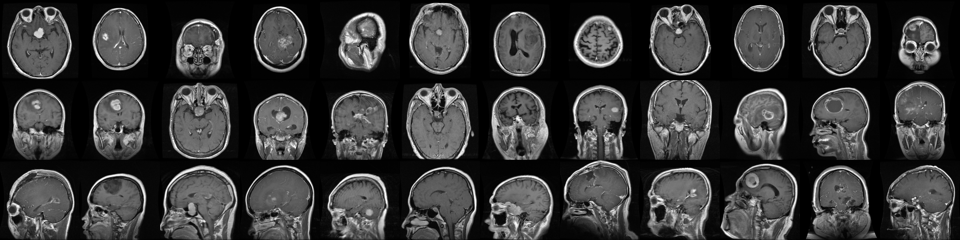
\includegraphics[width=\textwidth,keepaspectratio=true]{./fig/beyin_kesit_yonu_tahmini}
 \caption{Tahmin edilen kesit yönlerinden rastgele örnekler (satırlar: aksiyel, koronal, sagital). Görsel denetimde sagital grubun 12 örneğin 12'si, aksiyel grubun yaklaşık 9--10'u, koronal grubun yaklaşık 8'i doğru bulunmuştur.}
 \label{fig:yon}
\end{figure}

\section{Saldırı B: Açık Bağlamın Sızıntısı}\label{sec:res:B}

Çizelge \ref{tbl:saldiriB}, sunucunun gördüğü görüntüyle eğitilen CNN saldırganının sonuçlarını göstermektedir.

\begin{table*}[h!]
{\setlength{\tabcolsep}{4pt}
\caption{Bağlam saldırısında görüşe göre gizli alan oranı ve saldırgan AUC değeri ($\pm$ olan satırlar 5 tohumun ortalaması ve standart sapması, diğerleri tek tohumdur). Gizli alan tüm görüntülerin ortalamasıdır; beyin MR görüntüleri yalnızca görünür piksellerle normalize edilmiştir.}
\begin{center}
\vspace{-6mm}
{\small
\begin{tabular}{lcccc}
\hline\hline
& \multicolumn{2}{c}{Beyin MR (tümör tipi)} & \multicolumn{2}{c}{COVID-QU-Ex (teşhis)} \\
Görüş & Gizli alan & AUC & Gizli alan & AUC \\
\hline
Tam (şifresiz) & 0.000 & $0.9843 \pm 0.0012$ & 0.000 & $0.9966 \pm 0.0002$ \\
Yalnız ROI & 0.983 & 0.9683 & 0.765 & 0.9905 \\
Bağlam ($\Pi_{\mathrm{ROI}}$ görüşü) & 0.017 & $0.9759 \pm 0.0007$ & 0.235 & $0.9932 \pm 0.0001$ \\
Bağlam + 10 piksel & 0.051 & 0.9705 & 0.425 & 0.9915 \\
Bağlam + 20 piksel & 0.101 & 0.9663 & 0.609 & 0.9890 \\
Bağlam + 40 piksel & 0.248 & $0.9674 \pm 0.0016$ & 0.874 & $0.9556 \pm 0.0012$ \\
ROI sınırlayıcı kutusu & 0.025 & 0.9735 & 0.513 & 0.9839 \\
\hline
\end{tabular}}
\vspace{-6mm}
\end{center}
\label{tbl:saldiriB}}
\end{table*}

Her iki veri kümesinde de ROI'nin gizlenmesi saldırıyı neredeyse hiç zayıflatmamıştır. Beyin MR verisinde AUC $0.984$'ten $0.976$'ya, göğüs röntgeninde $0.997$'den $0.993$'e inmiştir; 5 tohumda standart sapma $0.002$'nin altındadır. Göğüs röntgeninde akciğerler 40 piksel genişletilerek görüntünün \%87'si gizlendiğinde bile AUC $0.956$ kalmış, normal ile pnömoni ayrımı $0.950$ olmuştur. Yalnızca ROI'nin görüldüğü referans görüşte AUC değerlerinin ($0.968$ ve $0.990$) bağlam görüşüyle aynı düzeyde olması, ROI dışındaki bağlamın teşhis için ROI'nin kendisi kadar bilgi taşıdığını göstermektedir.

\textbf{Normalizasyon denetimi.} Tezin ilk taslağında beyin MR kesitleri tüm pikselleriyle (tümör dahil) normalize edilmişti. Bu düzen aynı görüşlerde neredeyse aynı sonucu vermiştir: 5 tohumda tam görüşte $0.9852 \pm 0.0006$, bağlam görüşünde $0.9765 \pm 0.0009$, bağlam + 40 piksel görüşünde $0.9671 \pm 0.0021$ ve tek tohumlu görüşlerde en fazla $0.001$ fark. Yalnız ROI referansı ise $0.978$'den $0.968$'e inmiştir; tümör kendi pikselleriyle ölçeklendiğinde çevresine göre parlaklığı kaybolduğu için bu düşüş beklenir. Normalizasyon kanalının kendisi de ölçülmüştür. Tümörün eklenmesi, kesitlerin yalnızca \%2.5'inde yüzdelik aralığını \%1'den, \%0.03'ünde \%5'ten fazla değiştirmiştir; tümör çoğu kesitte en parlak doku değildir. Bu oran tümör tipini tek başına AUC $0.642$ ile tahmin etse de tümör alanıyla güçlü biçimde ilişkilidir (Spearman $-0.72$). Tümör alanı tek başına $0.653$, ikisi birlikte $0.669$ vermektedir; yani kanal, zaten açık olan ROI boyutunun ötesinde çok az bilgi taşır ve bağlam saldırısının başarısını açıklamaz.

\section{Gerçekçilik Testi}\label{sec:res:transfer}

Kaggle görüntülerine akciğer maskesi üretmek için eğitilen U-Net, COVID-QU-Ex doğrulama bölmesinde Dice benzerliği $0.978$'e ulaşmıştır. Üretilen 6.432 maskenin hiçbirinde akciğer alanı görüntünün \%5'inden küçük çıkmamış, maskeler görsel denetimde de doğru bulunmuştur (Şekil \ref{fig:maske}). Tekrar eden görüntüler çıkarıldıktan sonra Kaggle kümesinde 340 normal ve 1.157 pnömoni görüntüsü kalmıştır. Çizelge \ref{tbl:transfer} kümeler arası sonuçları vermektedir.

\begin{table*}[h!]
{\setlength{\tabcolsep}{3pt}
\caption{Saldırganın farklı bir kaynaktan veriyle eğitildiği gerçekçilik testi (normal / pnömoni, AUC ve \%95 GA).}
\begin{center}
\vspace{-6mm}
{\footnotesize
\begin{tabular}{lcccc}
\hline\hline
Eğitim $\rightarrow$ test & Eğitim & Test & Tam görüntü & Akciğer gizli \\
\hline
COVID-QU-Ex $\rightarrow$ Kaggle & 17.571 & 1.497 & 0.999 (0.998--1.000) & 0.998 (0.996--0.999) \\
Kaggle $\rightarrow$ COVID-QU-Ex & 1.215 & 4.393 & 0.928 (0.921--0.936) & 0.934 (0.928--0.941) \\
COVID-QU-Ex $\rightarrow$ COVID-QU-Ex & 17.571 & 4.393 & 0.992 & 0.984 \\
\hline
\end{tabular}}
\vspace{-6mm}
\end{center}
\label{tbl:transfer}}
\end{table*}

Hastanenin verisine hiç erişmeden, başka bir kaynaktan eğitilen saldırgan akciğerlerin şifreli olduğu görüntülerde pnömoniyi AUC $0.934$--$0.998$ ile bulmuştur. Küçük Kaggle kümesiyle eğitilen saldırganın akciğerler gizliyken daha iyi genellemesi ($0.928$'e karşı $0.934$), kaynaklar arasında taşınan bilginin önemli bölümünün akciğer dışında olduğuna işaret etmektedir. Kaggle kümesindeki normal ve pnömoni görüntüleri ile COVID-QU-Ex'in bir bölümü aynı çocuk hastalar kaynağından derlendiği için, bu test tamamen bağımsız bir hastane testi değildir (Bölüm \ref{sec:sinirliliklar}).

\begin{figure}[h!]
 \centering
 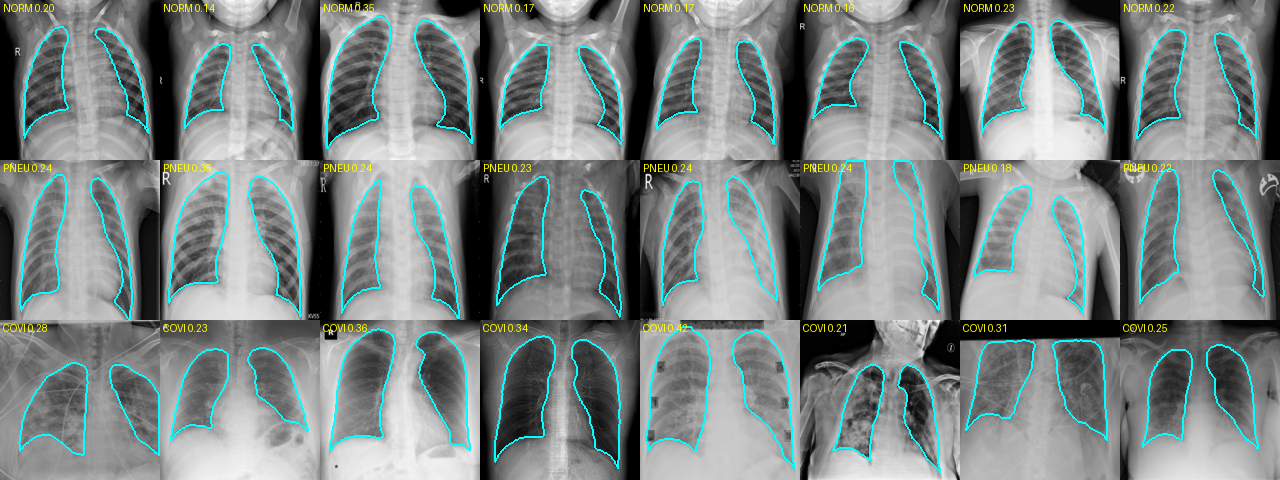
\includegraphics[width=\textwidth,keepaspectratio=true]{./fig/kaggle_akciger_maskeleri_kontrol}
 \caption{Kaggle göğüs röntgenlerine U-Net ile üretilen akciğer maskelerinden rastgele örnekler (satırlar: normal, pnömoni, COVID-19; sayı akciğer alanı oranıdır).}
 \label{fig:maske}
\end{figure}

\section{Sızıntının Kaynağı}\label{sec:res:root}

Çizelge \ref{tbl:gradcamcxr} ve Çizelge \ref{tbl:gradcambeyin}, bağlam görüşüyle eğitilen saldırganın Grad-CAM dikkat kütlesinin bölgelere dağılımını göstermektedir. Ortalama haritalar Şekil \ref{fig:camcxr} ve Şekil \ref{fig:cambeyin}'te verilmiştir.

\begin{table*}[h!]
{\setlength{\tabcolsep}{3pt}
\caption{Göğüs röntgeninde Grad-CAM dikkat kütlesinin bölgelere dağılımı (test bölmesinden 1500 görüntü; boş çıkan 1 harita paylara katılmamıştır).}
\begin{center}
\vspace{-6mm}
{\footnotesize
\begin{tabular}{lcccccc}
\hline\hline
Sınıf & Akciğer (gizli) & Kenar çerçeve & Akciğer üstü & Akciğer altı & Akciğerler arası & Yanlar \\
\hline
COVID-19 & 0.289 & 0.263 & 0.022 & 0.075 & 0.178 & 0.172 \\
Pnömoni & 0.256 & 0.270 & 0.031 & 0.059 & 0.184 & 0.200 \\
Normal & 0.286 & 0.265 & 0.039 & 0.048 & 0.216 & 0.146 \\
Tümü & 0.277 & 0.266 & 0.031 & 0.061 & 0.192 & 0.173 \\
\hline
\end{tabular}}
\vspace{-6mm}
\end{center}
\label{tbl:gradcamcxr}}
\end{table*}

\begin{table*}[h!]
{\setlength{\tabcolsep}{7pt}
\caption{Beyin MR görüntüsünde Grad-CAM dikkat kütlesinin bölgelere dağılımı (test katındaki 643 görüntü; meningiom görüntülerinden boş çıkan 13 harita paylara katılmamıştır).}
\begin{center}
\vspace{-6mm}
\begin{tabular}{lcccc}
\hline\hline
Sınıf & Tümör (gizli) & Tümör çevresi & Beynin geri kalanı & Arka plan \\
\hline
Meningiom & 0.033 & 0.101 & 0.513 & 0.353 \\
Gliom & 0.031 & 0.097 & 0.428 & 0.444 \\
Hipofiz & 0.024 & 0.125 & 0.720 & 0.131 \\
Tümü & 0.029 & 0.106 & 0.537 & 0.328 \\
\hline
\end{tabular}
\vspace{-6mm}
\end{center}
\label{tbl:gradcambeyin}}
\end{table*}

Göğüs röntgeninde saldırganın dikkati akciğerin dışında geniş bir bağlama yayılmıştır: kenar çerçeve (\%27), kalp ve mediasteni içeren akciğerler arası bölge (\%19) ve göğüs yanları (\%17). Normal sınıfında akciğerler arası bölgenin payı daha yüksektir (\%22). Gizli akciğer bölgesinin de \%28 pay alması iki nedene bağlanmaktadır. Birincisi, son evrişim bloğundaki $7 \times 7$ çözünürlüklü haritanın büyütülürken sınırlardan taşmasıdır. İkincisi, saldırganın gösterge kanalı üzerinden akciğerin şeklini kullanabilmesidir. Beyin MR görüntüsünde dikkatin yarısından fazlası beynin geri kalanında (\%54), yaklaşık üçte biri kafa dışı arka plandadır (\%33). Gliom ve meningiom sınıflarında arka planın payının yüksek olması (\%35--44), görüntüleme alanına veya cihaza özgü izlerin de sızıntıya katkı sağladığına işaret etmektedir. Bu yorum Bölüm \ref{sec:res:defense}'daki savunma bulgusuyla da tutarlıdır: kafa dışında açık kalan 8 piksel bile tümör tipini ele vermektedir.

Hedef sınıf skoru son blok etkinlikleriyle artmadığında Grad-CAM haritası tümüyle sıfır çıkar. Beyin MR verisinde meningiom görüntülerinin 166'sından 13'ünde, göğüs röntgeninde 1500 görüntünün 1'inde harita boş çıkmış ve bu haritalar bölge paylarına katılmamıştır. Tezin ilk taslağında boş haritalar sıfır paylarla ortalamaya girdiği için meningiom satırının toplamı $0.916$ görünüyordu; düzeltilmiş çizelgelerde her satırın toplamı $1$'dir.

\begin{figure}[h!]
 \centering
 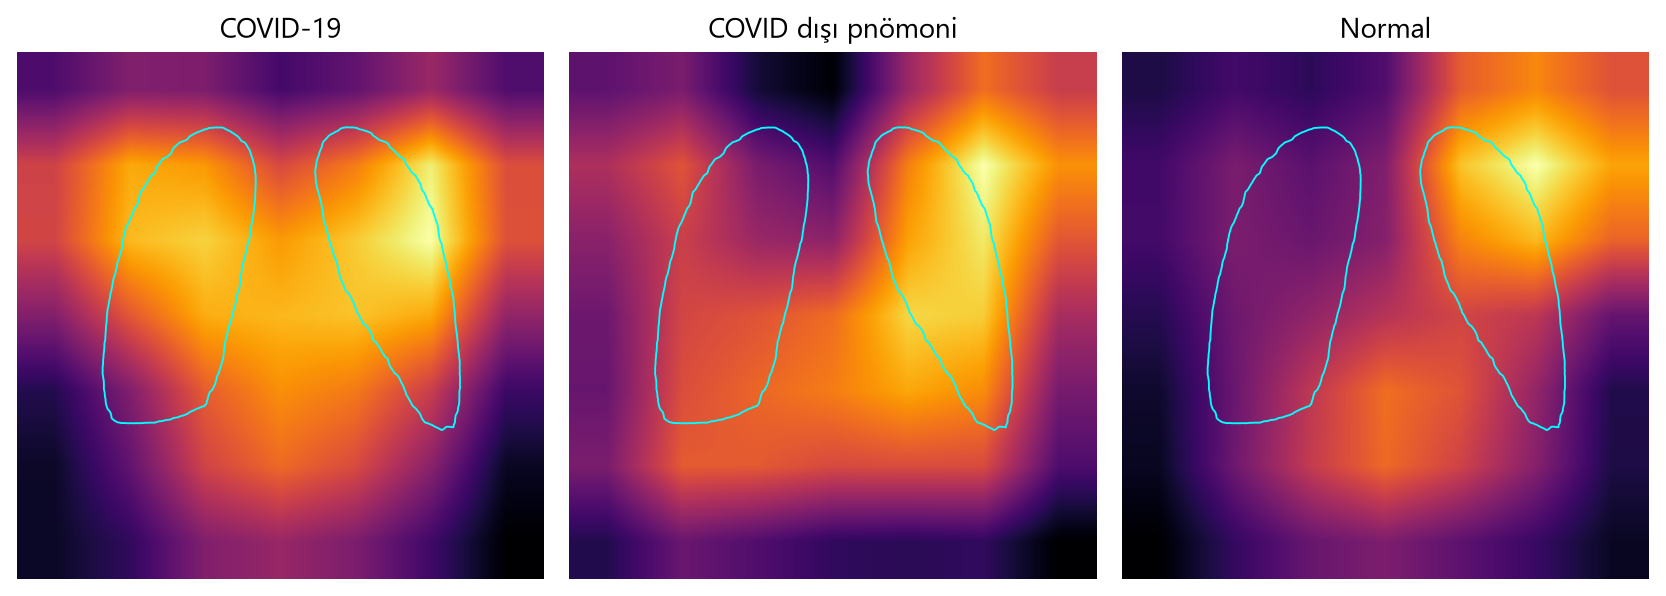
\includegraphics[width=\textwidth,keepaspectratio=true]{./fig/kok_neden_gradcam_covidqu_gnorm.png}
 \caption{COVID-QU-Ex verisinde akciğerler gizliyken saldırganın sınıf bazında ortalama Grad-CAM haritaları (açık renk yüksek dikkat; camgöbeği çizgi ortalama akciğer sınırıdır).}
 \label{fig:camcxr}
\end{figure}

\begin{figure}[h!]
 \centering
 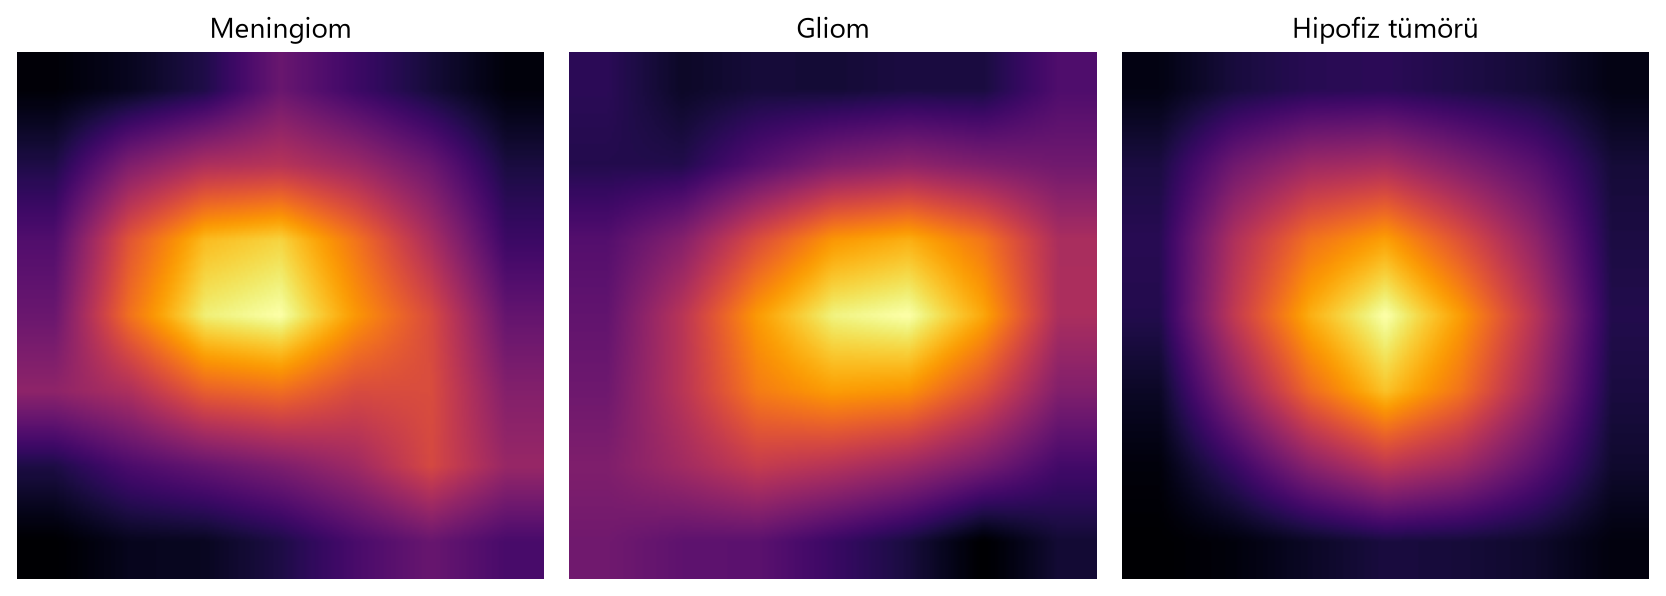
\includegraphics[width=\textwidth,keepaspectratio=true]{./fig/kok_neden_gradcam_brain_gnorm.png}
 \caption{Beyin MR verisinde tümör gizliyken saldırganın sınıf bazında ortalama Grad-CAM haritaları (açık renk yüksek dikkat; tümörlerin konumu görüntüler arasında değiştiği için ortalama sınır çizilmemiştir).}
 \label{fig:cambeyin}
\end{figure}

Çizelge \ref{tbl:onisleme}, önişleme adımlarının sızıntıya etkisini göstermektedir. Histogram eşitleme ve kenarın gizlenmesi saldırıyı anlamlı ölçüde zayıflatmamış, en güçlü birleşim bile AUC'yi yalnızca $0.993$'ten $0.988$'e indirmiştir. Sızıntı, basit önişlemeyle temizlenebilecek yüzeysel bir iz değildir.

\begin{table*}[h!]
{\setlength{\tabcolsep}{14pt}
\caption{COVID-QU-Ex verisinde önişleme adımlarının bağlam saldırısına etkisi (3 sınıf AUC).}
\begin{center}
\vspace{-6mm}
\begin{tabular}{lc}
\hline\hline
Önişleme & AUC \\
\hline
Yok & 0.993 \\
Histogram eşitleme & 0.993 \\
Dış kenarın \%5'inin gizlenmesi & 0.993 \\
Dış kenarın \%10'unun gizlenmesi & 0.990 \\
Histogram eşitleme ve \%10 kenar gizleme & 0.988 \\
\hline
\end{tabular}
\vspace{-6mm}
\end{center}
\label{tbl:onisleme}}
\end{table*}

\section{Savunmalar ve Gizlilik Şartlı Maliyet}\label{sec:res:defense}

Çizelge \ref{tbl:savunma}, savunma politikalarının seçilmiş noktalarını; Şekil \ref{fig:savcxr} ve Şekil \ref{fig:savbeyin} ise tüm eğrileri göstermektedir. Tamamen gizli kontrol görüşünde her iki veri kümesinde de AUC $0.500$ bulunmuş ve değerlendirme boru hattının doğru çalıştığı doğrulanmıştır.

\begin{table*}[h!]
{\setlength{\tabcolsep}{4pt}
\caption{Savunma politikalarında şifreli alan oranı (test görüntülerinin ortalaması), saldırgan AUC değeri ve protokol maliyetine göre hız kazancı (kat).}
\begin{center}
\vspace{-6mm}
{\small
\begin{tabular}{llcccc}
\hline\hline
Veri & Politika & $\rho$ & AUC & Hız ($256^2$) & Hız ($512^2$) \\
\hline
COVID-QU-Ex & Varsayılan ROI (akciğer) & 0.234 & 0.990 & 3.85 & 4.10 \\
 & Kanonik ROI & 0.633 & 0.974 & 1.47 & 1.57 \\
 & Kanonik ROI + 16 piksel & 0.911 & 0.910 & 1.00 & 1.09 \\
 & Sızıntı-güdümlü, 4. adım & 0.827 & 0.919 & 1.09 & 1.20 \\
 & Sızıntı-güdümlü, 9. adım & 0.981 & 0.776 & 1.00 & 1.02 \\
 & Kanonik ROI + 32 piksel & 0.996 & 0.681 & 1.00 & 1.00 \\
 & Tamamen gizli (kontrol) & 1.000 & 0.500 & 1.00 & 1.00 \\
\hline
Beyin MR & Varsayılan ROI (tümör) & 0.016 & 0.937 & 7.86 & 24.21 \\
 & Kanonik ROI & 0.334 & 0.921 & 2.83 & 2.94 \\
 & Kanonik ROI + 32 piksel & 0.791 & 0.901 & 1.14 & 1.26 \\
 & Sızıntı-güdümlü, 10. adım & 0.879 & 0.878 & 1.03 & 1.13 \\
 & Sızıntı-güdümlü, 12. adım & 0.982 & 0.824 & 1.00 & 1.02 \\
 & Kanonik ROI + 64 piksel & 0.9998 & 0.765 & 1.00 & 1.00 \\
 & Tamamen gizli (kontrol) & 1.000 & 0.500 & 1.00 & 1.00 \\
\hline
\end{tabular}}
\vspace{-6mm}
\end{center}
\label{tbl:savunma}}
\end{table*}

$\Pi_{\mathrm{ROI}}$'nin varsayılan kullanımında hız kazancı, görüntülerin özgün boyutunda göğüs röntgeninde ($256 \times 256$) 3.9, beyin MR görüntüsünde ($512 \times 512$) 24 kattır; ancak teşhis neredeyse tamamen açıktadır (AUC $0.990$ ve $0.937$). Tüm görüntülerde aynı olan kanonik ROI, meta veri sızıntısını kapatsa da saldırıyı yalnızca $0.974$ ve $0.921$ düzeyine indirmiştir.

Saldırgan AUC'sini $0.8$'in altına indirmek için göğüs röntgeninde sızıntı-güdümlü politikanın 9. adımına, yani görüntünün \%98.1'inin şifrelenmesine (yalnızca 968 piksel açık) ihtiyaç duyulmuştur. Bu noktada hız kazancı $256 \times 256$ görüntüde 1.00, $512 \times 512$ görüntüde 1.02 kattır. Beyin MR verisinde sızıntı-güdümlü politika \%98.2 şifreli alanda (920 piksel açık) bile $0.824$'te kalmıştır. $0.8$ hedefi yalnızca kafa dışında 8 pikselin açık kaldığı kanonik ROI + 64 piksel görüşünde ($\rho = 0.9998$, AUC $0.765$) ve tam şifrelemede sağlanmıştır; iki noktada da hız kazancı 1.00 kattır. $0.7$ ve $0.6$ hedefleri pratikte yalnızca tam şifrelemeyle karşılanmıştır. Göğüs röntgeninde kanonik ROI + 32 piksel görüşü 190 açık piksel ile $0.681$'e inmiştir. Beyin MR verisinde kafa dışında açık kalan 8 pikselin tümör tipini AUC $0.765$ ile ele vermesi, sızıntının çekim koşullarına bağlı izler de taşıdığını göstermektedir. İlk taslaktaki kesit normalizasyonunda bu değer $0.619$ idi; yalnızca görünür piksellerle yapılan normalizasyon, muhtemelen arka plandaki gürültü düzeyi farklarını görünür kıldığı için bu noktada sızıntıyı artırmıştır.

Sızıntı-güdümlü seçim, göğüs röntgeninde aynı şifreli alanda rastgele yama seçiminden daha düşük AUC sağlamıştır; örneğin yaklaşık \%93 şifreli alanda $0.864$'e karşı $0.895$ ve $0.920$. Beyin MR verisinde ise tutarlı bir üstünlük görülmemiştir: yaklaşık \%93 şifreli alanda güdümlü seçim $0.857$, rastgele sıralar $0.880$ ve $0.877$ vermiş; yaklaşık \%74'te ise güdümlü seçim ($0.904$) rastgele sıralardan ($0.888$ ve $0.886$) daha yüksek kalmıştır. Bu karşılaştırma tek tohumla, azaltılmış eğitim verisiyle ve $8 \times 8$ yama ızgarasıyla yapıldığından politikalar arasındaki birkaç puanlık farklar belirsizdir ve yalnızca eğilim olarak yorumlanmalıdır. Savunma saldırganları hesaplama maliyetini sınırlamak için daha az veriyle eğitildiğinden, gerçek sızıntının bu değerlerden de yüksek olması beklenir.

\begin{figure}[h!]
 \centering
 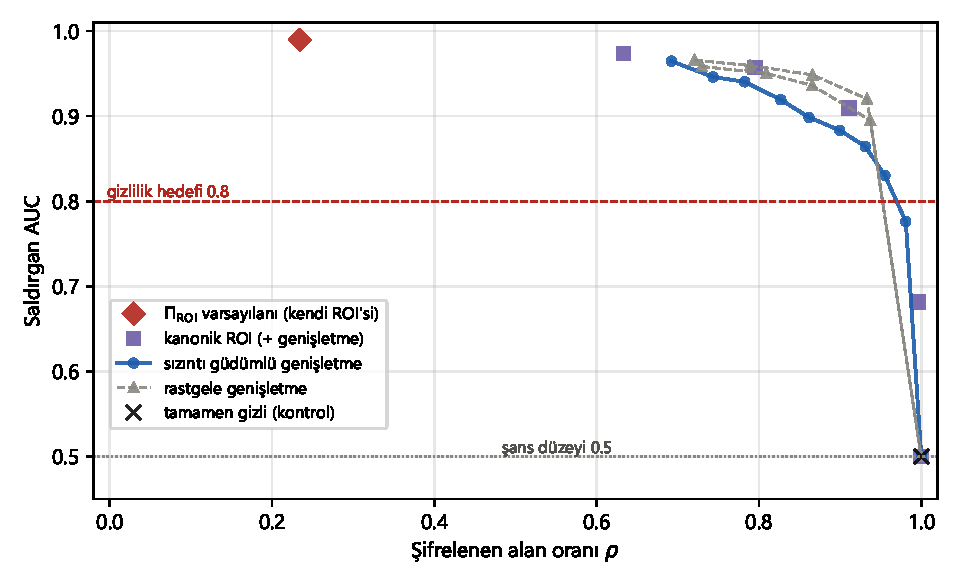
\includegraphics[width=12cm,keepaspectratio=true]{./fig/savunma_covidqu_tez.pdf}
 \caption{COVID-QU-Ex verisinde savunma politikalarının şifreli alan oranına göre saldırgan AUC eğrileri (kırmızı kesikli çizgi $0.8$ gizlilik hedefi, gri noktalı çizgi şans düzeyidir).}
 \label{fig:savcxr}
\end{figure}

\begin{figure}[h!]
 \centering
 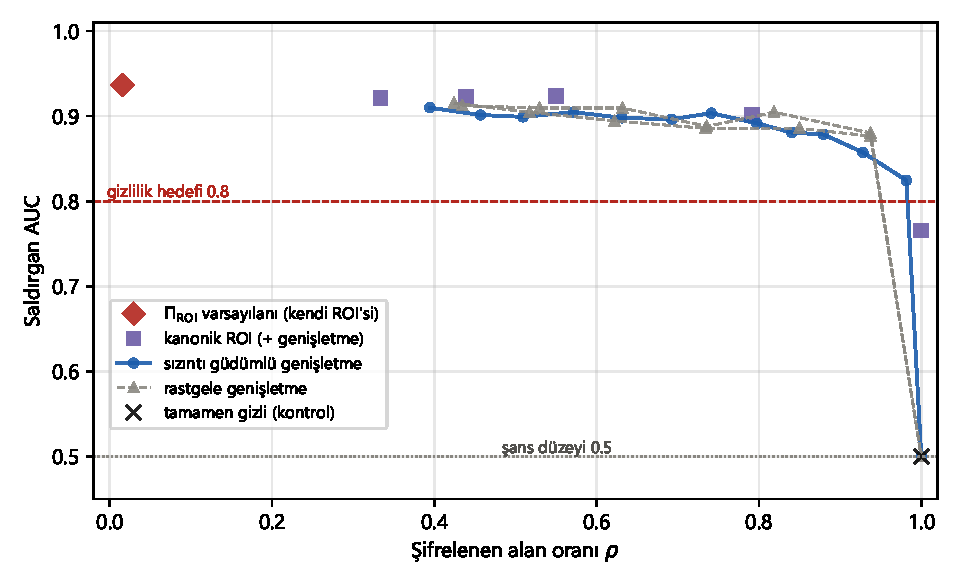
\includegraphics[width=12cm,keepaspectratio=true]{./fig/savunma_brain_tez.pdf}
 \caption{Beyin MR verisinde savunma politikalarının şifreli alan oranına göre saldırgan AUC eğrileri (çizgiler Şekil \ref{fig:savcxr} ile aynıdır).}
 \label{fig:savbeyin}
\end{figure}

\section{Odaklı Temsilde Teşhis Bilgisinin Korunması}\label{sec:res:fovinfo}

Çizelge \ref{tbl:fovbilgi}, odaklı temsillerin ve referansların ResNet-18 ile ölçülen teşhis başarısını göstermektedir. Seçilen iki yapılandırma da bilgi kaybı ölçütünü ($\leq 0.02$) her iki veri kümesinde tek bir şifreli metne sığarak karşılamıştır. Beyin MR verisinde odaklı temsiller tam görüntünün üstüne çıkmıştır: tam görüntü $0.9841$, F32\_G16 $0.9919$, F64\_G32 $0.9936$. Göğüs röntgeninde kayıp en fazla $0.0027$'dir.

\begin{table*}[h!]
{\setlength{\tabcolsep}{3pt}
\caption{Odaklı temsil ve referansların ResNet-18 ile ölçülen teşhis başarısı (makro AUC, 5 tohumun ortalaması ve standart sapması). Kayıp, aynı tohumdaki tam görüntüye göre farktır; negatif değer kazanç demektir.}
\begin{center}
\vspace{-6mm}
{\footnotesize
\begin{tabular}{lccccc}
\hline\hline
& & \multicolumn{2}{c}{Beyin MR (tümör tipi)} & \multicolumn{2}{c}{COVID-QU-Ex (teşhis)} \\
Temsil & Değer & AUC & Kayıp & AUC & Kayıp \\
\hline
Tam görüntü (224 piksel) & 50.176 & $0.9841 \pm 0.0011$ & -- & $0.9964 \pm 0.0001$ & -- \\
Tam görüntü + ROI penceresi & 50.179 & $0.9909 \pm 0.0011$ & $-0.0068$ & -- & -- \\
F32\_G16 & 1.283 & $0.9919 \pm 0.0009$ & $-0.0078$ & $0.9937 \pm 0.0001$ & $0.0027$ \\
F64\_G32 & 5.123 & $0.9936 \pm 0.0006$ & $-0.0095$ & $0.9951 \pm 0.0003$ & $0.0013$ \\
U32 & 1.024 & $0.9793 \pm 0.0015$ & $0.0048$ & $0.9940 \pm 0.0002$ & $0.0024$ \\
U32 + ROI penceresi & 1.027 & $0.9880 \pm 0.0011$ & $-0.0039$ & -- & -- \\
U64 & 4.096 & $0.9844 \pm 0.0009$ & $-0.0003$ & $0.9950 \pm 0.0002$ & $0.0014$ \\
U64 + ROI penceresi & 4.099 & $0.9893 \pm 0.0011$ & $-0.0052$ & -- & -- \\
U90 & 8.100 & $0.9866 \pm 0.0017$ & $-0.0025$ & -- & -- \\
U90 + ROI penceresi & 8.103 & $0.9910 \pm 0.0014$ & $-0.0069$ & -- & -- \\
\hline
\end{tabular}}
\vspace{-6mm}
\end{center}
\label{tbl:fovbilgi}}
\end{table*}

Beyin MR verisindeki kazancın kaynağı ROI penceresi referanslarıyla ayrıştırılmıştır. Tam görüntüye yalnızca pencerenin konumunu gösteren kanal eklendiğinde AUC $0.9909$'a çıkmış ve artış 5 tohumun 5'inde görülmüştür; yani kazancın büyük bölümü ROI'nin konum ve boyut bilgisinden gelmektedir. Buna karşın aynı konum bilgisi verildiğinde de odaklı temsil eş bütçeli küçültmenin önünde kalmıştır. F32\_G16, U32 + ROI penceresinden $0.0039$; F64\_G32, U64 + ROI penceresinden $0.0043$ ve tam görüntü + ROI penceresinden $0.0027$ daha yüksektir ve fark her üç karşılaştırmada 5 tohumun 5'inde aynı yöndedir. Çözünürlüğün odağa verilmesinin katkısı küçük ama tutarlıdır ve tam görüntünün yaklaşık 10 ile 40 katı daha az değerle elde edilmektedir.

Göğüs röntgeninde akciğer penceresi görüntünün neredeyse tamamını kapsadığından odaklı temsil eş bütçeli küçültmeyle aynı sonucu vermiştir: F32\_G16 ile U32 arasındaki fark $-0.0003$, F64\_G32 ile U64 arasındaki fark $0.0001$'dir. Şekil \ref{fig:fovbilgi}, tek tohumla taranan tüm yapılandırmaları şifrelenen değer sayısına göre göstermektedir.

\begin{figure}[h!]
 \centering
 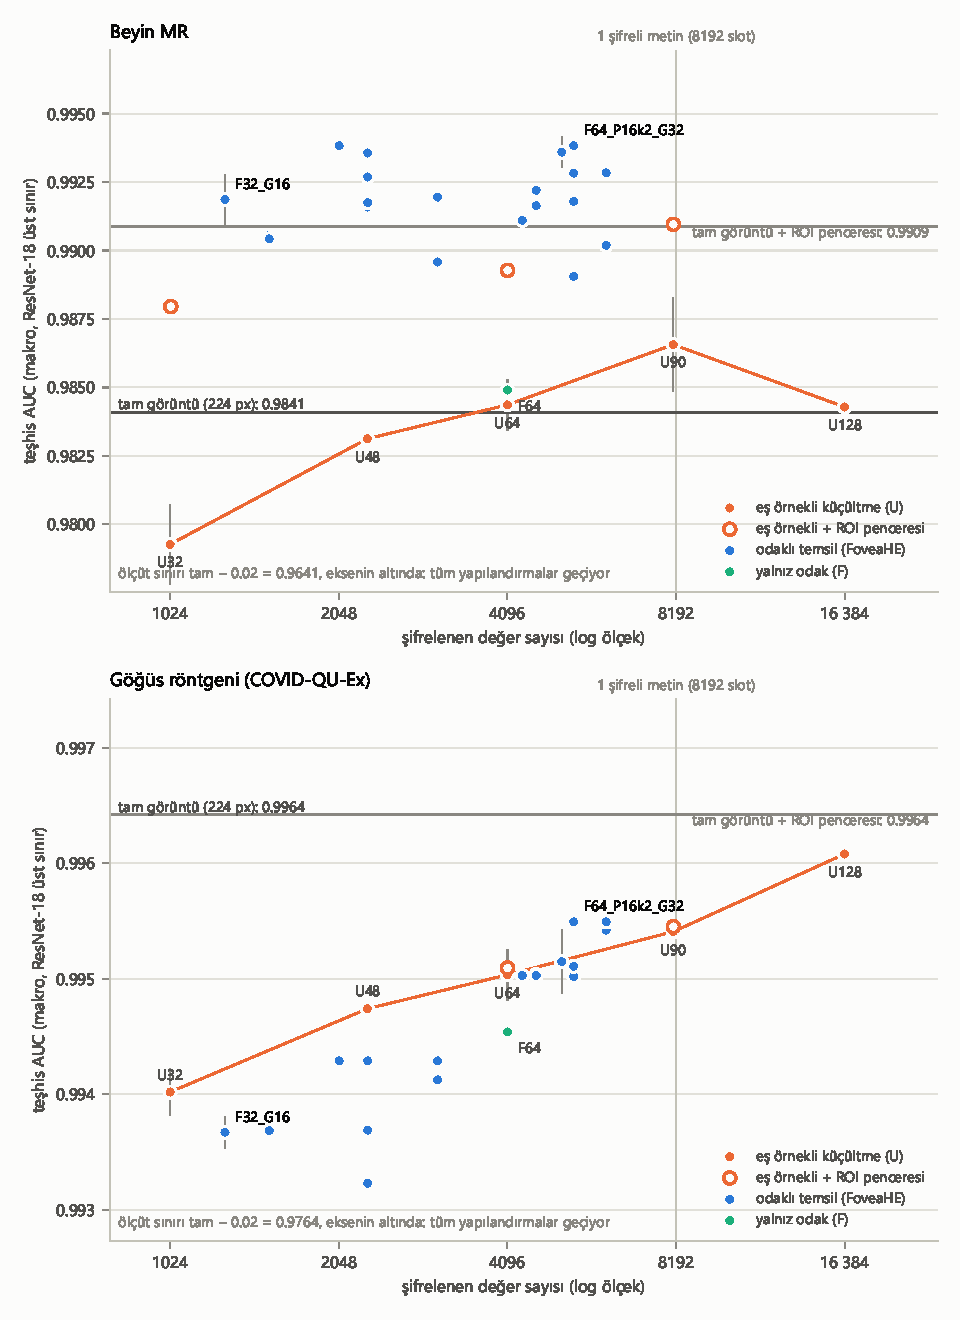
\includegraphics[width=13cm,keepaspectratio=true]{./fig/cozum_bilgi_egrisi_tez.pdf}
 \caption{Şifrelenen değer sayısına göre ResNet-18 ile ölçülen teşhis AUC değeri (üstte beyin MR, altta COVID-QU-Ex). Mavi noktalar odaklı temsilleri, turuncu çizgi eş örnekli küçültmeyi, içi boş turuncu işaretler ROI penceresi referanslarını, yeşil noktalar yalnız odak temsillerini gösterir. Yatay çizgiler tam görüntü ve tam görüntü + ROI penceresi değerleri, dikey çizgi tek şifreli metnin kapasitesidir. Hata çubukları 5 tohumun standart sapmasıdır; hata çubuğu olmayan noktalar tek tohumludur. Yapılandırma adlarında F odak, P yakın çevre ($k$: pencerenin odağa göre büyütme katsayısı), G genel bakış katmanının kenar uzunluğudur; örneğin F64\_P16k2\_G32, $64 \times 64$ odak, 2 kat büyük pencereden $16 \times 16$ yakın çevre ve $32 \times 32$ genel bakış demektir (Bölüm \ref{sec:fov:rep}).}
 \label{fig:fovbilgi}
\end{figure}

\section{Şifreli Çalışabilen Modellerin Teşhis Başarısı}\label{sec:res:fovmodel}

Çizelge \ref{tbl:fovmodel}, şifreli çalışabilen modellerin 5 tohumlu teşhis başarısını göstermektedir. Seçici şifreleme model çıktısını değiştirmediği için tam görüntü sütunundaki Model D değeri $\Pi_{\mathrm{ROI}}$ protokolünün teşhis başarısıdır. Model kaybı ölçütü ($\leq 0.03$) iki veri kümesinde, üç model sınıfında ve iki yapılandırmada karşılanmış; odaklı temsil her durumda tam görüntünün üstüne çıkmıştır.

\begin{table*}[h!]
{\setlength{\tabcolsep}{3pt}
\caption{Şifreli çalışabilen modellerin temsile göre teşhis başarısı (makro AUC, 5 tohumun ortalaması ve standart sapması). Tam görüntü, beyin MR verisinde $512 \times 512$, göğüs röntgeninde $256 \times 256$ piksel özgün çözünürlüktür. U64 + geometri, U64'e odaklı temsilin üç geometri değerinin eklendiği referanstır.}
\begin{center}
\vspace{-6mm}
{\footnotesize
\begin{tabular}{llccccc}
\hline\hline
Veri & Model & Tam görüntü & F32\_G16 & F64\_G32 & U64 & U64 + geometri \\
\hline
Beyin MR & D & $0.881 \pm 0.004$ & $0.948 \pm 0.001$ & $0.945 \pm 0.002$ & $0.882 \pm 0.002$ & $0.882 \pm 0.003$ \\
 & D2 & $0.872 \pm 0.006$ & $0.909 \pm 0.006$ & $0.910 \pm 0.005$ & $0.864 \pm 0.005$ & $0.860 \pm 0.009$ \\
 & C & $0.852 \pm 0.008$ & $0.944 \pm 0.006$ & $0.927 \pm 0.014$ & $0.848 \pm 0.008$ & $0.851 \pm 0.007$ \\
\hline
COVID-QU-Ex & D & $0.895 \pm 0.006$ & $0.915 \pm 0.002$ & $0.915 \pm 0.002$ & $0.865 \pm 0.002$ & $0.867 \pm 0.002$ \\
 & D2 & $0.946 \pm 0.001$ & $0.954 \pm 0.002$ & $0.952 \pm 0.001$ & $0.938 \pm 0.002$ & $0.937 \pm 0.001$ \\
 & C & $0.925 \pm 0.009$ & $0.930 \pm 0.002$ & $0.935 \pm 0.002$ & $0.917 \pm 0.004$ & $0.919 \pm 0.005$ \\
\hline
\end{tabular}}
\vspace{-6mm}
\end{center}
\label{tbl:fovmodel}}
\end{table*}

Kazanç beyin MR verisinde büyüktür: Model D'de $0.881$'den $0.948$'e, Model C'de $0.852$'den $0.944$'e yükselmiştir. Göğüs röntgeninde en başarılı model sınıfı olan D2'de başarı $0.946$'dan $0.954$'e çıkmıştır. Eş bütçeli küçültme (U64) ise tam görüntünün önüne geçememiş, göğüs röntgeninde Model D'de tam görüntünün $0.030$ gerisinde kalmıştır. Ayar aramasında hiçbir seçim arama sınırına dayanmamış, aktarılan ağırlıklar ile eğitilmiş model arasındaki en büyük fark $10^{-4}$'ün altında kalmıştır.

FoveaHE'ye ROI'nin konumu ve boyutu istemcideki maskeden verildiği için kazancın ne kadarının ``modele ROI'nin yerini söylemekten'' geldiği ayrıca sınanmıştır. U64'e FoveaHE'nin üç geometri değeri eklendiğinde başarı hiçbir model sınıfında belirgin biçimde artmamıştır: U64 ile ortalama farkın mutlak değeri beyin MR verisinde en fazla $0.004$, göğüs röntgeninde en fazla $0.002$'dir. Aynı ROI bilgisine sahip bu referansla karşılaştırıldığında FoveaHE F32\_G16 beyin MR verisinde $0.048$--$0.093$, göğüs röntgeninde $0.011$--$0.048$ daha başarılıdır (eşleştirilmiş, tohum bazında fark) ve fark iki veri kümesinde, üç model sınıfında ve iki yapılandırmada 5 tohumun 5'inde aynı yöndedir. Dolayısıyla sığ modellerde kazanç, ROI konumunun sayı olarak verilmesinden değil, ROI istemcide bilindiğinde çözünürlüğün ROI'ye ayrılmasından gelmektedir: sığ modeller ROI'yi kendi başlarına bulamaz ve üç sayıdan yararlanarak doğru pikselleri seçemez; odaklı temsil ise ROI'yi modele merkezlenmiş ve yüksek çözünürlüklü olarak sunar.

\section{Şifreli Çıkarımın Doğruluğu ve Maliyeti}\label{sec:res:fovcost}

Şifreli çıkarım şifresiz çıkarımla aynı sonucu vermiştir. İki veri kümesinde, üç model sınıfında ve üç yapılandırmada test bölmesinden seçilen 120 görüntüde en büyük logit farkı $1.6 \times 10^{-4}$, tahmin uyumu \%100 ve AUC farkı $0$ bulunmuş; şifreli doğruluk ölçütü ($\leq 0.005$) karşılanmıştır.

Çizelge \ref{tbl:fovcost} maliyet dökümünü vermektedir. FoveaHE temsili Model D ve D2'de tek bir şifreli metne, Model C'de katman başına bir şifreli metne sığdığı için sunucu süresi görüntü boyutundan bağımsızdır: Model D ve D2'de yaklaşık 1.2--1.5 saniye, Model C'de yaklaşık 0.5 saniye. Tam şifrelemeye göre hız kazancı Model D ve D2'de beyin MR görüntüsünde 29--37 kat, göğüs röntgeninde 7--9 kattır. Model C'de tam şifreleme zaten daha ucuz olduğundan kazanç beyin MR görüntüsünde 18--21 kat, göğüs röntgeninde 4.4--5.3 kattır. Hız ölçütü ($\geq 5$) göğüs röntgeninde Model C'nin F64\_G32 yapılandırması (4.4 kat) dışında tüm satırlarda karşılanmıştır. İstemciden sunucuya giden veri 27.4 MB ve 6.8 MB'tan 0.9--1.7 MB'a inmiş, istemci tarafında temsilin çıkarılması ana yapılandırmalarda görüntü başına 4--12 milisaniye sürmüştür.

Bu hız kazancının kaynağı odaklama değil, temsilin boyutudur. Aynı ölçüm düzeninde şifreli çalıştırılan eş örnekli U64 de tek bir şifreli metne sığmış ve benzer hız kazancı vermiştir: Model D'de beyin MR görüntüsünde 33.3, göğüs röntgeninde 7.8 kat. Tek şifreli metne sığan her temsil bu hızı alır; FoveaHE'nin katkısı, aynı bütçede doğruluğu korumaktır (Bölüm \ref{sec:res:fovmodel}). Göğüs röntgeninde gizlilik şartlı $\Pi_{\mathrm{ROI}}$ (\%98 şifreli alan) tam şifrelemeyle aynı süreyi vermiştir. Tam şifreleme süreleri Çizelge \ref{tbl:maliyet}'deki yeniden üretim ölçümünden farklı bir ölçüm oturumuna aittir; hız kazançları her zaman aynı oturumda ölçülen tam şifreleme süresine göre hesaplanmıştır.

\begin{table*}[h!]
{\setlength{\tabcolsep}{4pt}
\caption{Şifreli çıkarımın maliyet dökümü (3 tekrarın ortalaması, bilgisayarda başka iş yokken). Süreler saniye, yükleme boyutu MB cinsindendir; hız kazancı aynı model sınıfında tam şifrelemeye göredir.}
\begin{center}
\vspace{-6mm}
{\footnotesize
\begin{tabular}{llcccccc}
\hline\hline
Yöntem & Model & Değer & Şifreli metin & Sunucu & Toplam & Yükleme & Hız \\
\hline
\multicolumn{8}{l}{\emph{Beyin MR}} \\
Tam şifreleme & D & 262.144 & 32 & 44.10 & 44.46 & 27.38 & 1.0 \\
FoveaHE F32\_G16 & D & 1.283 & 1 & 1.20 & 1.21 & 0.86 & 36.6 \\
FoveaHE F64\_G32 & D & 5.123 & 1 & 1.38 & 1.40 & 0.86 & 31.8 \\
FoveaHE F32\_G16 & D2 & 1.283 & 1 & 1.27 & 1.28 & 0.86 & 34.8 \\
FoveaHE F64\_G32 & D2 & 5.123 & 1 & 1.52 & 1.53 & 0.86 & 29.0 \\
Tam şifreleme & C & 262.144 & 32 & 9.76 & 10.16 & 27.39 & 1.0 \\
FoveaHE F32\_G16 & C & 1.280 & 2 & 0.46 & 0.48 & 1.71 & 21.3 \\
FoveaHE F64\_G32 & C & 5.120 & 2 & 0.55 & 0.58 & 1.71 & 17.6 \\
\hline
\multicolumn{8}{l}{\emph{COVID-QU-Ex}} \\
Tam şifreleme & D & 65.536 & 8 & 10.27 & 10.36 & 6.85 & 1.0 \\
$\Pi_{\mathrm{ROI}}$, \%98 şifreli & D & 64.009 & 8 & 10.22 & 10.30 & 6.85 & 1.0 \\
FoveaHE F32\_G16 & D & 1.283 & 1 & 1.17 & 1.19 & 0.86 & 8.7 \\
FoveaHE F64\_G32 & D & 5.123 & 1 & 1.42 & 1.44 & 0.86 & 7.2 \\
FoveaHE F32\_G16 & D2 & 1.283 & 1 & 1.28 & 1.30 & 0.86 & 8.0 \\
FoveaHE F64\_G32 & D2 & 5.123 & 1 & 1.47 & 1.49 & 0.86 & 7.0 \\
Tam şifreleme & C & 65.536 & 8 & 2.41 & 2.51 & 6.85 & 1.0 \\
FoveaHE F32\_G16 & C & 1.280 & 2 & 0.45 & 0.47 & 1.71 & 5.3 \\
FoveaHE F64\_G32 & C & 5.120 & 2 & 0.54 & 0.57 & 1.71 & 4.4 \\
\hline
\end{tabular}}
\vspace{-6mm}
\end{center}
\label{tbl:fovcost}}
\end{table*}

\section{FoveaHE Sızıntı Denetimi}\label{sec:res:fovleak}

Çizelge \ref{tbl:fovleak}, sunucunun gördüğü bilgilerle kurulan saldırganların sonuçlarını göstermektedir. FoveaHE'de şifreli metin sayısı, slot sayısı ve yükleme boyutu tanım gereği her görüntüde aynıdır ve CKKS işlemleri veriden bağımsızdır. Bu nedenle FoveaHE satırlarının şans düzeyinde çıkması beklenen bir sonucun doğrulanmasıdır: paket meta verisi ve yan kanal saldırganlarının kat ortalamalı AUC değeri $0.448$--$0.526$ aralığında kalmış, hiçbiri etiket permütasyonlarıyla elde edilen boş dağılımın \%95'lik sınırını aşmamıştır ($p \geq 0.20$). Ölçümün asıl anlamı sunucu süresi gibi uygulamaya bağlı yan kanallarda, özellikle de denetimin sızıntıyı yakalayabildiğini gösteren pozitif kontroldedir. Sızıntı ölçütü ($\leq 0.55$) iki veri kümesinde de karşılanmıştır.

Aynı örneklemde ve aynı yöntemle değerlendirilen $\Pi_{\mathrm{ROI}}$ paket meta verisi ise yalnızca şifreli metin sayısı ve yükleme boyutuyla bile şans düzeyinden anlamlı olarak ayrılmıştır ($0.557$--$0.589$, $p < 0.01$). Bu pozitif kontrol, denetimin gerçek bir sızıntıyı yakalayabildiğini göstermektedir. $\Pi_{\mathrm{ROI}}$ değerlerinin Saldırı A'dan ($0.83$) düşük olmasının nedeni, burada ROI geometrisi yerine yalnızca paket düzeyinde gözlenebilen kaba bilgilerin kullanılmasıdır. FoveaHE'de açık piksel olmadığından bağlam saldırısı uygulanamaz.

\begin{table*}[h!]
{\setlength{\tabcolsep}{3pt}
\caption{Sunucunun gördüğü bilgilerle sızıntı denetimi (5 tohum, sınıf dengeli katlar, kat ortalamalı AUC, 100 etiket permütasyonuyla boş dağılımın \%95'lik sınırı ve $p$ değeri).}
\begin{center}
\vspace{-6mm}
{\footnotesize
\begin{tabular}{lllp{3.6cm}cccc}
\hline\hline
Veri & Yöntem & Tür & Öznitelikler & $n$ & AUC & Boş \%95 & $p$ \\
\hline
Beyin MR & $\Pi_{\mathrm{ROI}}$ & Paket & Şifreli metin sayısı, yükleme boyutu & 3.064 & 0.561 & 0.509 & $<0.01$ \\
 & FoveaHE & Paket & Şifreli metin ve slot sayısı, yükleme boyutu & 3.064 & 0.491 & 0.520 & 0.85 \\
 & $\Pi_{\mathrm{ROI}}$ & Yan kanal & Şifreli metin sayısı, yükleme boyutu & 450 & 0.557 & 0.520 & $<0.01$ \\
 & FoveaHE & Yan kanal & Sunucu süresi, yanıt boyutu & 450 & 0.526 & 0.546 & 0.20 \\
 & FoveaHE & Yan kanal & Yalnızca sunucu süresi & 450 & 0.484 & 0.540 & 0.73 \\
\hline
COVID-QU-Ex & $\Pi_{\mathrm{ROI}}$ & Paket & Şifreli metin sayısı, yükleme boyutu & 3.000 & 0.573 & 0.514 & $<0.01$ \\
 & FoveaHE & Paket & Şifreli metin ve slot sayısı, yükleme boyutu & 3.000 & 0.503 & 0.518 & 0.43 \\
 & $\Pi_{\mathrm{ROI}}$ & Yan kanal & Şifreli metin sayısı, yükleme boyutu & 450 & 0.589 & 0.533 & $<0.01$ \\
 & FoveaHE & Yan kanal & Sunucu süresi, yanıt boyutu & 450 & 0.468 & 0.535 & 0.84 \\
 & FoveaHE & Yan kanal & Yalnızca sunucu süresi & 450 & 0.448 & 0.533 & 0.98 \\
\hline
\end{tabular}}
\vspace{-6mm}
\end{center}
\label{tbl:fovleak}}
\end{table*}

\section{Rakip Yaklaşımlar}\label{sec:res:rivals}

\textbf{Şifreli özet.} Çizelge \ref{tbl:rakipler}, şifreli özet yaklaşımını FoveaHE ile karşılaştırmaktadır. Şifreli özet de açık piksel ve değişken meta veri içermez ve sunucu süresi FoveaHE ile aynı düzeydedir (yaklaşık 1 saniye). Doğrulukta ise iki veri kümesinde de FoveaHE'nin önündedir: beyin MR verisinde $0.955$'e karşı $0.948$ (eşleştirilmiş fark $0.007 \pm 0.002$), göğüs röntgeninde $0.982$'ye karşı $0.954$ (eşleştirilmiş, tohum bazında fark $0.027 \pm 0.002$; ortalamaların farkı yuvarlamadan dolayı $0.028$ görünür). Fark her iki veri kümesinde 5 tohumun 5'inde aynı yöndedir. Buna karşılık şifreli özet, istemcide 11.2 milyon parametreli bir ağın çalıştırılmasını gerektirir: işlemcide görüntü başına tüm çekirdeklerle 23, tek çekirdekle 51--55 milisaniye. FoveaHE'nin istemci işlemi ise yalnızca yeniden örneklemedir (ana yapılandırmalarda 4--12 milisaniye).

\begin{table*}[h!]
{\setlength{\tabcolsep}{4pt}
\caption{Şifreli özet ile FoveaHE'nin karşılaştırılması (AUC 5 tohumun ortalaması ve standart sapması; süreler tohum 0 ölçümüdür). İstemci süresinde parantez içindeki değer tek çekirdek süresidir.}
\begin{center}
\vspace{-6mm}
{\footnotesize
\begin{tabular}{lllcccc}
\hline\hline
Veri & Yöntem & Model & Değer & AUC & Süre (s) & İstemci (ms) \\
\hline
Beyin MR & FoveaHE F32\_G16 & D & 1.283 & $0.948 \pm 0.001$ & 1.21 & 10 \\
 & Şifreli özet & D & 512 & $0.955 \pm 0.001$ & 1.01 & 23 (55) \\
 & Şifreli özet & D2 & 512 & $0.946 \pm 0.004$ & 1.08 & 23 (55) \\
\hline
COVID-QU-Ex & FoveaHE F32\_G16 & D2 & 1.283 & $0.954 \pm 0.002$ & 1.30 & 4 \\
 & Şifreli özet & D & 512 & $0.968 \pm 0.001$ & 0.96 & 23 (51) \\
 & Şifreli özet & D2 & 512 & $0.982 \pm 0.001$ & 1.06 & 23 (51) \\
\hline
\end{tabular}}
\vspace{-6mm}
\end{center}
\label{tbl:rakipler}}
\end{table*}

\textbf{Bozuk bağlam.} Çizelge \ref{tbl:gurultu}, açık bağlamın gürültü veya bulanıklıkla bozulduğu durumu göstermektedir. Bozulma sızıntıyı durdurmamıştır. En güçlü gürültüde ($\sigma = 0.4$) saldırgan AUC değeri beyin MR verisinde $0.967$, göğüs röntgeninde $0.983$ olmuş; bozulmasız bağlam saldırısına göre ($0.976$ ve $0.993$) düşüş en fazla $0.01$ kalmıştır. Aynı bozulmada ROI'nin temiz olduğu görüşte fayda da korunmuştur ($0.987$ ve $0.993$). Saldırgan bozulmaya uyum sağladığında bağlamdaki teşhis izi kaybolmamaktadır.

\begin{table*}[h!]
{\setlength{\tabcolsep}{6pt}
\caption{Bozuk bağlam deneyi (tek tohum): saldırgan AUC (ROI gizli, bağlam bozuk) ve fayda AUC (ROI temiz, bağlam bozuk).}
\begin{center}
\vspace{-6mm}
\begin{tabular}{lcccc}
\hline\hline
& \multicolumn{2}{c}{Beyin MR} & \multicolumn{2}{c}{COVID-QU-Ex} \\
Bozulma & Saldırgan & Fayda & Saldırgan & Fayda \\
\hline
Yok (5 tohum, Çizelge \ref{tbl:saldiriB}) & 0.976 & 0.984 & 0.993 & 0.997 \\
Gauss gürültüsü, $\sigma = 0.05$ & 0.973 & 0.990 & 0.992 & 0.996 \\
Gauss gürültüsü, $\sigma = 0.10$ & 0.972 & 0.989 & 0.989 & 0.995 \\
Gauss gürültüsü, $\sigma = 0.20$ & 0.971 & 0.988 & 0.986 & 0.995 \\
Gauss gürültüsü, $\sigma = 0.40$ & 0.967 & 0.987 & 0.983 & 0.993 \\
Gauss bulanıklığı, $\sigma = 2$ piksel & 0.977 & 0.993 & 0.992 & 0.996 \\
Gauss bulanıklığı, $\sigma = 4$ piksel & 0.981 & 0.993 & 0.991 & 0.996 \\
Gauss bulanıklığı, $\sigma = 8$ piksel & 0.977 & 0.994 & 0.988 & 0.994 \\
\hline
\end{tabular}
\vspace{-6mm}
\end{center}
\label{tbl:gurultu}}
\end{table*}

\section{Beş Yaklaşımın Karşılaştırması}\label{sec:res:compare}

Çizelge \ref{tbl:karsilastirma}, Şekil \ref{fig:paretobeyin} ve Şekil \ref{fig:paretocxr}, beş yaklaşımı teşhis başarısı, hız ve saldırgan başarısı açısından birlikte göstermektedir. Her satırda o temsil için 5 tohumda en başarılı model sınıfının değeri verilmiştir (beyin MR verisinde Model D, göğüs röntgeninde Model D2). Hız, aynı model sınıfının tam şifreleme süresine göredir. Tamamen şifreli yöntemlerde sunucunun gördüğü veri boyutu sabit olduğundan, saldırgan değeri olarak FoveaHE denetimindeki en yüksek AUC verilmiştir. $\Pi_{\mathrm{ROI}}$ satırlarında saldırgan değeri bağlam saldırısından, gizlilik şartlı satırda ise tanım gereği $0.8$ sınırından gelmektedir. Bu satırların hızları savunma deneyindeki şifreli alan oranlarından ve görüntülerin özgün boyutundaki (beyin MR $512 \times 512$, göğüs röntgeni $256 \times 256$) maliyet ölçümünden, göğüs röntgeninde gizlilik şartlı satır için ise doğrudan ölçümden hesaplanmıştır. Beyin MR verisinde gizlilik şartlı nokta pratikte tam şifrelemedir: $0.8$ koşulunu sağlayan iki nokta, yalnızca 8 pikselin açık kaldığı görüş (saldırgan $0.765$) ve tam şifrelemedir (saldırgan $0.50$); ikisinde de hız kazancı 1.00 kattır. Bozuk bağlam satırında doğruluk ve hız $\Pi_{\mathrm{ROI}}$ varsayılanıyla aynı kabul edilmiştir.

\begin{table*}[h!]
{\setlength{\tabcolsep}{4pt}
\caption{Beş yaklaşımın karşılaştırılması: teşhis AUC (5 tohum ortalaması), tam şifrelemeye göre hız kazancı (kat) ve sunucunun gördüğü bilgilerle saldırgan AUC.}
\begin{center}
\vspace{-6mm}
{\small
\begin{tabular}{lcccccc}
\hline\hline
& \multicolumn{3}{c}{Beyin MR} & \multicolumn{3}{c}{COVID-QU-Ex} \\
Yöntem & AUC & Hız & Saldırgan & AUC & Hız & Saldırgan \\
\hline
Tam şifreleme & 0.881 & 1.0 & 0.53 & 0.946 & 1.0 & 0.50 \\
$\Pi_{\mathrm{ROI}}$, varsayılan ROI & 0.881 & 24.2 & 0.98 & 0.946 & 3.9 & 0.99 \\
$\Pi_{\mathrm{ROI}}$, gizlilik şartlı & 0.881 & 1.0 & 0.80 & 0.946 & 1.0 & 0.80 \\
Bozuk bağlam ($\sigma = 0.4$) & 0.881 & 24.2 & 0.97 & 0.946 & 3.9 & 0.98 \\
FoveaHE F32\_G16 & 0.948 & 36.6 & 0.53 & 0.954 & 8.0 & 0.50 \\
FoveaHE F64\_G32 & 0.945 & 31.8 & 0.53 & 0.952 & 7.0 & 0.50 \\
Şifreli özet & 0.955 & 44.0 & 0.53 & 0.982 & 9.8 & 0.50 \\
\hline
\end{tabular}}
\vspace{-6mm}
\end{center}
\label{tbl:karsilastirma}}
\end{table*}

Karşılaştırma üç sonucu bir arada göstermektedir. Birincisi, $\Pi_{\mathrm{ROI}}$'nin hızı gizlilikle birlikte var olamamaktadır: saldırgan $0.8$'in altına indirildiğinde hız kazancı beyin MR görüntüsünde 24.2 kattan 1.0 kata, göğüs röntgeninde 3.9 kattan 1.0 kata inmektedir. İkincisi, bağlamı bozmak hızı korusa da sızıntıyı gidermemektedir. Üçüncüsü, tamamen şifreli iki yaklaşım olan FoveaHE ve şifreli özet, saldırganı şans düzeyinde tutarken tam şifrelemeden hem çok daha hızlı hem daha doğrudur. FoveaHE beyin MR görüntüsünde 36.6 kat hızla $0.948$, göğüs röntgeninde 8.0 kat hızla $0.954$ AUC'ye ulaşmıştır; şifreli özet her iki veri kümesinde de daha doğrudur.

\begin{figure}[h!]
 \centering
 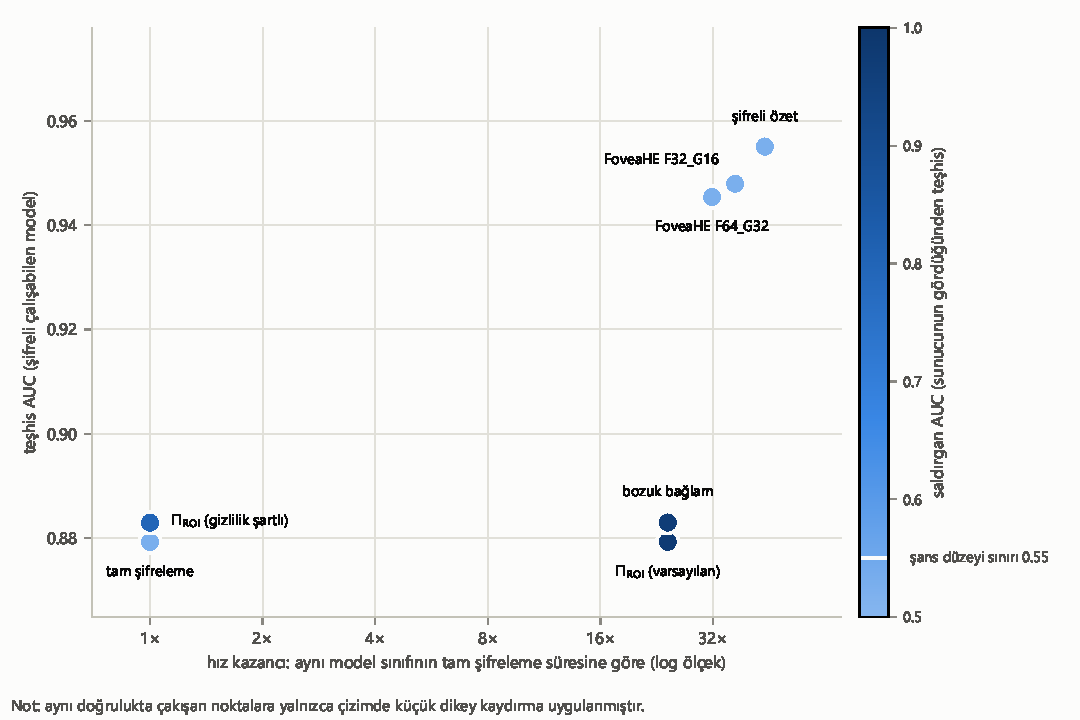
\includegraphics[width=12.5cm,keepaspectratio=true]{./fig/cozum_pareto_brain.pdf}
 \caption{Beyin MR verisinde beş yaklaşımın teşhis AUC değeri, tam şifrelemeye göre hız kazancı (logaritmik ölçek) ve saldırgan AUC değeri (renk; koyu renk yüksek sızıntı demektir). Aynı doğruluktaki çakışan noktalar yalnızca çizimde dikey olarak hafifçe kaydırılmıştır.}
 \label{fig:paretobeyin}
\end{figure}

\begin{figure}[h!]
 \centering
 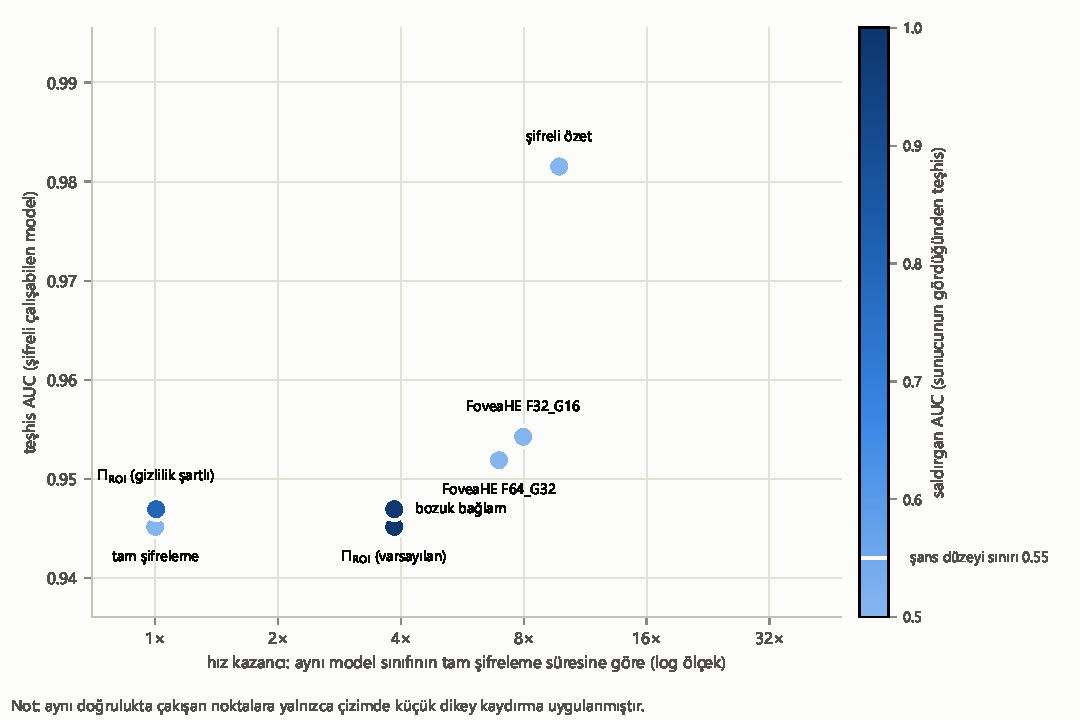
\includegraphics[width=12.5cm,keepaspectratio=true]{./fig/cozum_pareto_covidqu.pdf}
 \caption{COVID-QU-Ex verisinde beş yaklaşımın teşhis AUC değeri, hız kazancı ve saldırgan AUC değeri (Şekil \ref{fig:paretobeyin} ile aynı gösterim).}
 \label{fig:paretocxr}
\end{figure}

\section{Bütçe Duyarlı Odak}\label{sec:res:budget}

Çizelge \ref{tbl:butce} ve Şekil \ref{fig:butce}, sabit şifreli değer bütçesinde odak payının etkisini göstermektedir. Her bütçede, iki veri kümesinde ve iki model sınıfında odak ile genel bakışın birlikte kullanıldığı en iyi paylaşım, hem yalnız genel bakıştan (eş örnekli küçültme) hem yalnız odaktan daha başarılı olmuştur. Eş örnekli küçültmeye göre kazanç beyin MR verisinde Model C'de $0.090$--$0.109$, Model D'de $0.066$--$0.077$; göğüs röntgeninde Model D'de $0.046$--$0.061$, Model C'de $0.013$--$0.021$'dir. Yalnız odağa göre kazanç $0.014$--$0.081$ aralığındadır. En iyi sonuçlar $0.25$ ile $0.75$ arasındaki nominal odak paylarında elde edilmiştir; kenar uzunlukları tam sayıya yuvarlandığı için gerçekleşen paylar $0.24$--$0.76$ arasındadır.

Beyin MR verisinde bütçeyi büyütmek başarıyı artırmamış, en iyi sonuçlar $1.024$ ve $2.048$ değerle elde edilmiştir. Göğüs röntgeninde ise bütçe arttıkça küçük bir iyileşme görülmüştür. Bu deney tek tohumla yapıldığından, aynı bütçedeki komşu paylar arasındaki küçük farklar yorumlanmamalıdır.

\begin{table*}[h!]
{\setlength{\tabcolsep}{4pt}
\caption{Bütçe duyarlı odak (tek tohum, makro AUC): eş örnekli küçültme (odak payı 0), en iyi karışım, bu karışımın yapılandırması ve odak payı, yalnız odak (odak payı 1).}
\begin{center}
\vspace{-6mm}
{\footnotesize
\begin{tabular}{llcccccc}
\hline\hline
Veri & Model & Bütçe & Eş örnekli & En iyi karışım & Yapılandırma & Pay & Yalnız odak \\
\hline
Beyin MR & C & 1.024 & 0.855 & 0.952 & F27\_G17 & 0.71 & 0.915 \\
 &  & 2.048 & 0.847 & 0.955 & F39\_G22 & 0.76 & 0.892 \\
 &  & 4.096 & 0.849 & 0.939 & F45\_G45 & 0.50 & 0.876 \\
 &  & 8.192 & 0.847 & 0.939 & F78\_G45 & 0.75 & 0.892 \\
 & D & 1.024 & 0.879 & 0.956 & F16\_G27 & 0.26 & 0.881 \\
 &  & 2.048 & 0.884 & 0.950 & F32\_G31 & 0.52 & 0.871 \\
 &  & 4.096 & 0.879 & 0.949 & F45\_G45 & 0.50 & 0.869 \\
 &  & 8.192 & 0.881 & 0.951 & F45\_G78 & 0.25 & 0.870 \\
\hline
COVID-QU-Ex & C & 1.024 & 0.919 & 0.932 & F22\_G23 & 0.48 & 0.916 \\
 &  & 2.048 & 0.921 & 0.940 & F22\_G39 & 0.24 & 0.919 \\
 &  & 4.096 & 0.916 & 0.937 & F55\_G32 & 0.75 & 0.923 \\
 &  & 8.192 & 0.921 & 0.942 & F45\_G78 & 0.25 & 0.927 \\
 & D & 1.024 & 0.854 & 0.915 & F27\_G17 & 0.71 & 0.900 \\
 &  & 2.048 & 0.866 & 0.917 & F39\_G22 & 0.76 & 0.902 \\
 &  & 4.096 & 0.868 & 0.919 & F45\_G45 & 0.50 & 0.901 \\
 &  & 8.192 & 0.875 & 0.921 & F45\_G78 & 0.25 & 0.897 \\
\hline
\end{tabular}}
\vspace{-6mm}
\end{center}
\label{tbl:butce}}
\end{table*}

\begin{figure}[h!]
 \centering
 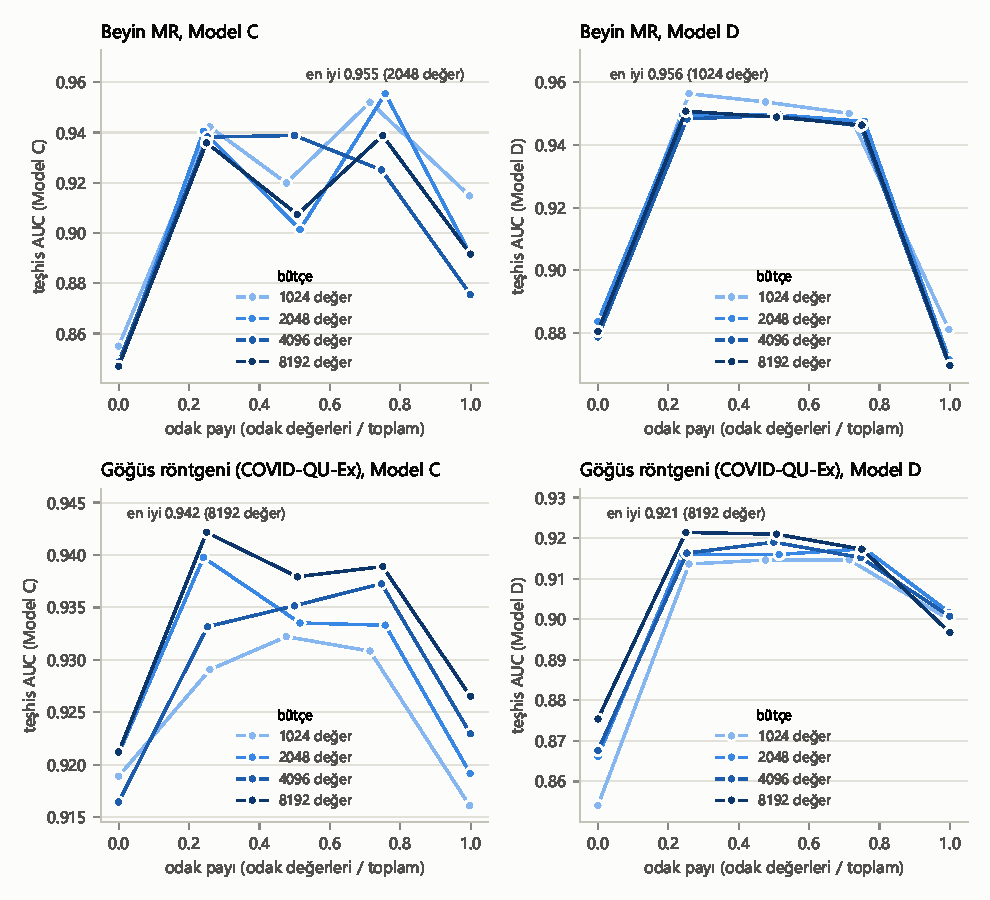
\includegraphics[width=14cm,keepaspectratio=true]{./fig/cozum_butce_tez.pdf}
 \caption{Bütçe duyarlı odak: her panelde bütçe başına (açıktan koyuya 1.024--8.192 değer) odak payına göre teşhis AUC değeri.}
 \label{fig:butce}
\end{figure}

\section{Harici Derlemede Genelleme}\label{sec:res:generalization}

Çizelge \ref{tbl:genelleme} ve Şekil \ref{fig:genelleme}, COVID-QU-Ex ile eğitilen modellerin yeniden eğitilmeden Kaggle kümesinde değerlendirilmesini göstermektedir. Temsiller arasındaki sıralama harici derlemede de korunmuştur. FoveaHE her model sınıfında tam görüntünün önündedir: eşleştirilmiş fark Model D'de $0.033$--$0.036$, Model C'de $0.015$--$0.017$, Model D2'de $0.005$--$0.006$'dır ve fark 30 karşılaştırmanın 29'unda aynı yöndedir. Eş bütçeli küçültme ise tam görüntünün gerisinde kalmıştır. Şifreli özet harici derlemede de en yüksek başarıyı vermiştir ($0.985$). Bu testte ROI, radyolog maskesi değil, U-Net'in ürettiği akciğer maskesidir; sıralamanın korunması, FoveaHE'nin kazancının kusursuz bir ROI'ye bağlı olmadığına kısmi bir kanıttır. Ancak göğüs röntgeninde ROI görüntünün büyük bölümünü kapsadığından, tümör gibi küçük ROI'lerde tahmin hatasının etkisi ayrıca incelenmelidir.

Piksel tabanlı temsillerin tamamında harici AUC iç AUC'den $0.02$--$0.04$ yüksektir. Bu durum, büyük ölçüde çocuk hastalara ait pnömoni görüntülerinden oluşan harici kümenin daha kolay ayrıştırıldığını göstermektedir. Bu nedenle sonuç mutlak bir genelleme kazancı olarak değil, temsiller arasındaki sıralamanın farklı bir derlemede korunması olarak yorumlanmalıdır.

\begin{table*}[h!]
{\setlength{\tabcolsep}{5pt}
\caption{COVID-QU-Ex ile eğitilen modellerin Kaggle kümesinde (tekrar etmeyen 1.767 görüntü) yeniden eğitilmeden değerlendirilmesi (makro AUC, 5 tohum). Son sütun aynı model ve tohumda tam görüntüye göre eşleştirilmiş farktır; parantez içinde farkın pozitif olduğu tohum sayısı verilmiştir.}
\begin{center}
\vspace{-6mm}
{\small
\begin{tabular}{lllccc}
\hline\hline
Temsil & Yapılandırma & Model & İç AUC & Harici AUC & Tam görüntüye göre fark \\
\hline
Tam görüntü & U256 & D & 0.895 & $0.914 \pm 0.011$ & -- \\
Tam görüntü & U256 & D2 & 0.946 & $0.973 \pm 0.002$ & -- \\
Tam görüntü & U256 & C & 0.925 & $0.945 \pm 0.005$ & -- \\
Eş örnekli & U64 & D & 0.865 & $0.892 \pm 0.019$ & $-0.022$ (0/5) \\
Eş örnekli & U64 & D2 & 0.938 & $0.971 \pm 0.003$ & $-0.002$ (2/5) \\
Eş örnekli & U64 & C & 0.917 & $0.942 \pm 0.004$ & $-0.003$ (2/5) \\
FoveaHE & F32\_G16 & D & 0.915 & $0.950 \pm 0.008$ & $0.036$ (5/5) \\
FoveaHE & F32\_G16 & D2 & 0.954 & $0.978 \pm 0.002$ & $0.005$ (5/5) \\
FoveaHE & F32\_G16 & C & 0.930 & $0.960 \pm 0.003$ & $0.015$ (5/5) \\
FoveaHE & F64\_G32 & D & 0.915 & $0.947 \pm 0.005$ & $0.033$ (5/5) \\
FoveaHE & F64\_G32 & D2 & 0.952 & $0.979 \pm 0.004$ & $0.006$ (4/5) \\
FoveaHE & F64\_G32 & C & 0.935 & $0.962 \pm 0.003$ & $0.017$ (5/5) \\
Şifreli özet & -- & D & 0.968 & $0.971 \pm 0.002$ & -- \\
Şifreli özet & -- & D2 & 0.982 & $0.985 \pm 0.002$ & -- \\
\hline
\end{tabular}}
\vspace{-6mm}
\end{center}
\label{tbl:genelleme}}
\end{table*}

\begin{figure}[h!]
 \centering
 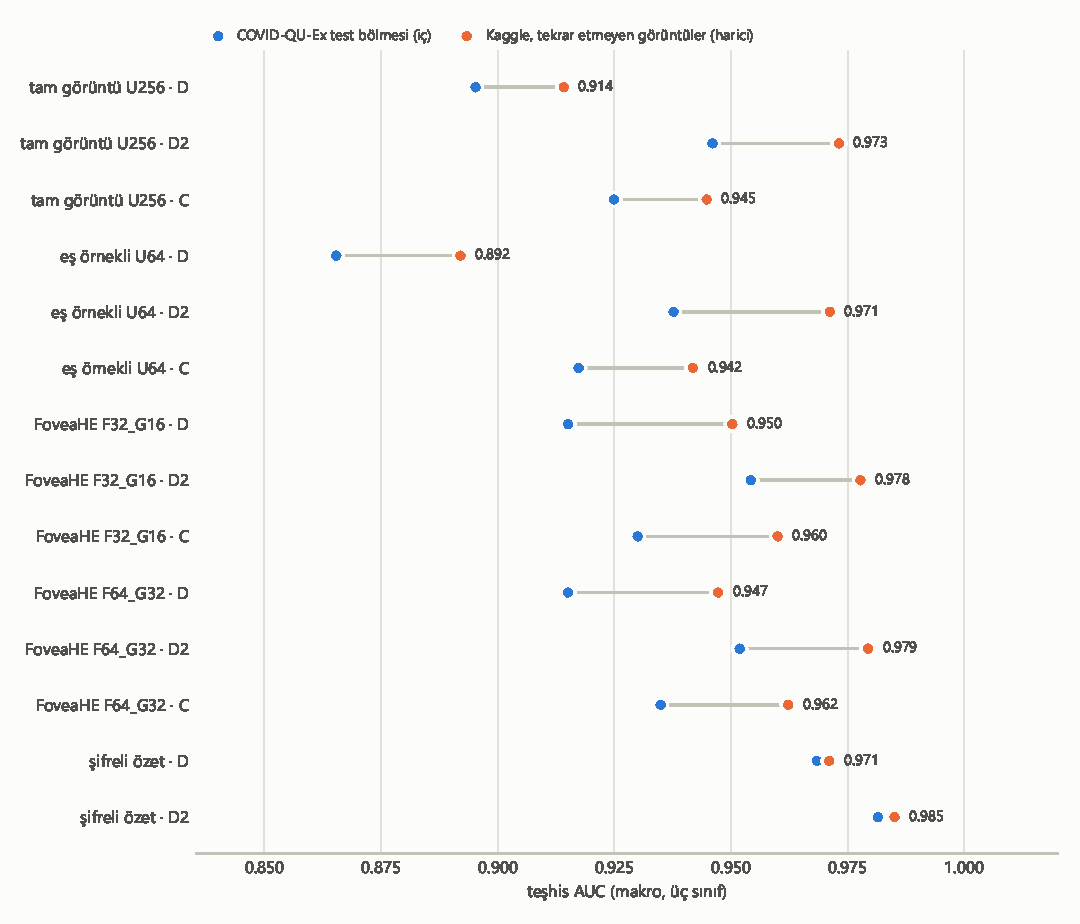
\includegraphics[width=12cm,keepaspectratio=true]{./fig/cozum_genelleme_tez.pdf}
 \caption{COVID-QU-Ex test bölmesindeki (iç, mavi) ve Kaggle kümesindeki (harici, turuncu) teşhis AUC değerleri (5 tohum ortalaması; etiketler harici değerdir).}
 \label{fig:genelleme}
\end{figure}
